\documentclass{article}

\usepackage[utf8]{inputenc}
\usepackage{amsthm}
\usepackage{amssymb}
\usepackage{mathtools}
\usepackage{graphicx}
\usepackage{mdframed}
\usepackage{float}
\usepackage[top=0.75in, bottom=0.75in, left=0.75in, right=0.75in]{geometry}
\usepackage{gauss}

\usepackage{array}
\allowdisplaybreaks

\makeatletter
\newcounter{elimination@steps}
\newcolumntype{R}[1]{>{\raggedleft\arraybackslash$}p{#1}<{$}}
\def\elimination@num@rights{}
\def\elimination@num@variables{}
\def\elimination@col@width{}
\newenvironment{elimination}[4][0]
{
    \setcounter{elimination@steps}{0}
    \def\elimination@num@rights{#1}
    \def\elimination@num@variables{#2}
    \def\elimination@col@width{#3}
    \renewcommand{\arraystretch}{#4}
    \start@align\@ne\st@rredtrue\m@ne
}
{
    \endalign
    \ignorespacesafterend
}
\newcommand{\step}[2]
{
    \ifnum\value{elimination@steps}>0\sim\quad\fi
    \left[
        \ifnum\elimination@num@rights>0
            \begin{array}
            {@{}*{\elimination@num@variables}{R{\elimination@col@width}}
            |@{}*{\elimination@num@rights}{R{\elimination@col@width}}}
        \else
            \begin{array}
            {@{}*{\elimination@num@variables}{R{\elimination@col@width}}}
        \fi
            #1
        \end{array}
    \right]
    & 
    \begin{array}{l}
        #2
    \end{array}
    \addtocounter{elimination@steps}{1}
}
\makeatother

\DeclarePairedDelimiter{\abs}{\lvert}{\rvert}
\DeclarePairedDelimiter{\norm}{\lvert \lvert}{\rvert \rvert}

\newtheoremstyle{break}% name
  {}%         Space above, empty = `usual value'
  {}%         Space below
  {\itshape}% Body font
  {}%         Indent amount (empty = no indent, \parindent = para indent)
  {\bfseries}% Thm head font
  {.}%        Punctuation after thm head
  {\newline}% Space after thm head: \newline = linebreak
  {}%         Thm head spec

\newtheorem{Def}{Definition}[section]

\theoremstyle{break}

\newtheorem{innerEx}{Exempel}[section]
\newtheorem{sats}{Sats}[section]
\newtheorem{Rem}{Anmärkning}[]

\newenvironment{Ex}
{\begin{mdframed} \begin{innerEx} \vspace{3pt}}
{\vspace{3pt} \end{innerEx} \end{mdframed}}  

\newenvironment{bevis}
{\begin{mdframed} \begin{proof} \vspace{3pt}}
{\vspace{3pt} \end{proof} \end{mdframed}}

\usepackage{color}
\usepackage{bnf}
\title{
	 Finite Automata Theory and Formal Languages\\
	 Föreläsning 1
    \author{Erik Sjöström}
}
\begin{document}
\maketitle

\section{Automata}
\label{sec:Automata}

\subsection{Dictionary definition}
\label{sub:Dictionary definition}
\emph{Main Entry:} $au \cdot tom \cdot a \cdot ton$\\
\emph{Function:} noun\\
\emph{Inflected Form(s):} plural $au \cdot tom \cdot atons$ or $au \cdot tom \cdot a \cdot ta$\\
\emph{Etymology:} Latin, from Greek, neuter of automatos\\
\emph{Date:} 1645
\begin{enumerate}
    \item a mechanism that is relatively self-operating;\\especially: robot
    \item a machine or control mechanism designed to follow automatically
    a predetermined sequense of operations or respond to encoded instructions
    \item an individual who acts in a mechanical fashion
\end{enumerate}

\subsection{Applications}
\label{sub:Applications}
Models for ...
\begin{itemize}
    \item Lexical analyser in a compiler
	\item Software for designing circuits
	\item Software for finding patterns in large bodies of text such as
	collections of web pages
	\item Software for verifying systems with a finit number of different
	states such as protocols
	\item Real machines like vending machines, telephones, street lights, ...
	\item Application in linguistics, building of large dictionary,
	spell programs, search
	\item Application in genetics, regular pattern in the language of protein
\end{itemize}

\subsection{Example: on/off-switch}
\label{sub:Example: on/off-switch}
A very simple finite automaton:
\begin{center}
	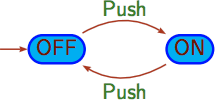
\includegraphics[scale=0.5]{onOff.png}
\end{center}
{\color{red} \emph{States}} represented by ``circles''.\\
One {\color{red} \emph{starting}} state, indicated with an arrow into it.\\
Labelled arc between states represent observable {\color{red} \emph{events}}.\\
Sometimes one of more {\color{red} \emph{final}} states,
indicated with a double circle: 
\includegraphics[scale=0.5]{doubleCircle.png}
\begin{center}
	
\includegraphics[scale=0.5]{doubleCircle.png}
\end{center}

\subsection{Example: Parity Counter}
\label{sub:Example: Parity Counter}
The states of an automaton can be thought of as its {\color{red} \emph{memory}}.\\
A finite-state automaton has {\color{red} \emph{finite memory}}!
\begin{center}
	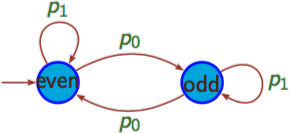
\includegraphics[scale=0.5]{parityCounter.png}
\end{center}
Two events: $p_0$ and $p_1$.\\
The machine does nothing on the event $p_1$.\\
The machine remembers the parity of the number of $p_0$'s.\\
\smallskip

\noindent
{\color{magenta} Correctnes:} We would like to prove that the automata is on
the state even \emph{iff} an even number of $p_0$ were pressed.

\subsection{Example: Vending Machines}
\label{sub:Example: Vending Machines}
A simple vending machine:
\begin{center}
	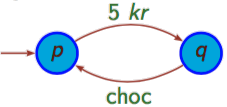
\includegraphics[scale=0.5]{vendingMachine.png}
\end{center}
What happens if we ask for chocolate on \emph{p}?\\
\smallskip

\noindent
\textbf{A more complex vending machine}:
\begin{center}
	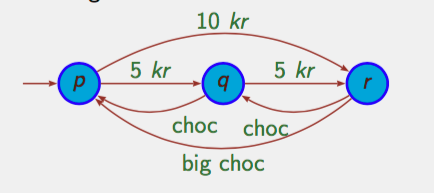
\includegraphics[scale=0.5]{complexVendingMachine.png}
\end{center}

\subsection{Example: The Man, the Wolf, the Goat, and the Cabbage}
\label{sub:Example: The Man, the Wolf, the Goat, and the Cabbage}
A man with a wolf, a goat and a cabbage is on the left bank of a river.\\
There is a boat large enough to carry the man and only one of the other
three things.\\
The man wants to move everything to the right bank.\\
However if the man leaves the wolf and the goat unattended on either
shore, the wolf surely will eat the goat.\\
Similarly, if the goat and the cabbage are left unattended,
the goat will eat the cabbage.\\
\smallskip

\noindent
{\color{magenta} \textbf{Problem}:} Is it possible to cross the river
without the goat or cabbage being eaten?\\
How many possible solutions does the problem have?\\
\smallskip

\noindent
{\color{magenta} \textbf{Solution}:} We design an automaton that models the problem
with all its possible transitions, and look for paths between the initial
and final state.
\begin{center}
	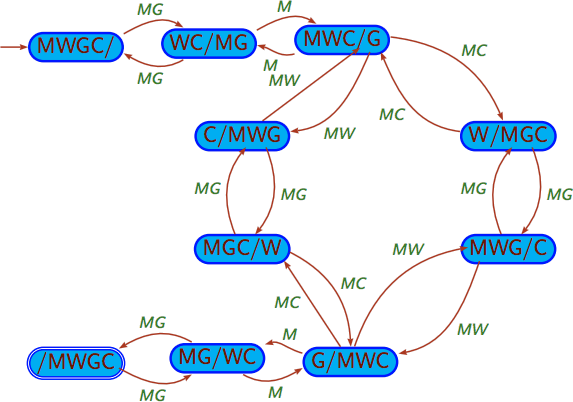
\includegraphics[scale=0.5]{boatRide.png}
\end{center}

\section{Formal Language}
\label{sec:Formal Language}

\subsection{From Wikipedia:}
\label{sub:From Wikipedia:}

In mathematics, computer science, and linguistics,
a formal language is a set of strings of symbols that may
be constrained by rules that are specific to it.\\
The alphabet of a formal language is the set of symbols,
letters, or tokens from which the strings of the language may be formed;
frequently it is required to be finite.\\
The strings formed from this alphabet are called words,
and the words that belong to a particular formal language
are sometimes called well-formed words or well-formed formulas.\\
A formal language is often defined by means of a formal
grammar such as a regular grammar or context-free grammar,
also called its formation rule.

\subsection{Example: Formal Representation of Numbers and Identifiers in a Programming Language}
\label{sub:Example: Formal Representation of Numbers and Identifiers in a Programming Language}

A regular grammar for numbers and identifiers:

\begin{grammar}
	[(colon){ $\rightarrow$ }]
	[(semicolon){ $|$ }]
	[(period){.}]
	L:A;B;...;Z;a;b;...;z\\
	D:0;1;2;3;4;5;6;7;8;9
\end{grammar}
\begin{grammar}
	[(colon){ $\rightarrow$ }]
	[(semicolon){ $|$ }]
	[(period){.}]
	Nr:D;D Nr\\
	Id:L LLoD\\
	LLoD:L LLoD;D LLoD;$\epsilon$
\end{grammar}
A regular expression for numbers:
\begin{grammar}
	(0 + 1 + 2 + 3 + 4 + 5 + 6 + 7 + 8 + 9)$^+$
\end{grammar}
A regular expression for identifiers:
\begin{grammar}
	[(period){.}]
	(A + ... + Z + a + ... + z)(A + ... + Z + a + ... + z + 0 + ... + 9)$^*$
\end{grammar}
\subsection{Example: Very Simple Expression}
\label{sub:Example: Very Simple Expression}
A context-free grammar for simple expression:
\begin{grammar}
	[(colon){ $\rightarrow$ }]
	[(semicolon){ $|$ }]
	[(period){...}]
	E:E+E;E-E;E*E;E/E;(E);Nr;Id\\
	Nr:.\\
	Id:.
\end{grammar}
{\color{magenta}Correctness:} We could want to prove that:
\begin{itemize}
	\item Any expression has as many ``('' as ``)''
	\item Any expression has 1 more ``term'' than the number of ``operations''
	\item ...
\end{itemize}

\subsection{More Complex Example}
\label{sub:More Complex Example}
A better context-free grammar for simple expression:
\begin{grammar}
	[(colon){ $\rightarrow$ }]
	[(semicolon){ $|$ }]
	[(period){...}]
	E:E+T;E-T;T\\
	T:T*F;T/F;F\\
	F:(E);Nr;Id
\end{grammar}
A context-free grammar for C++ compund statements:
\begin{grammar}
	[(colon){ $\rightarrow$ }]
	[(semicolon){ $|$ }]
	[(period){...}]
	[(quote){ \begin{bf}}{\end{bf}}]
	S:{LC}\\
	LC:$\epsilon$;C LC\\
	C:S;"if" (E) C;"if" (E) C"else" C;\\
	%men va fan, jävla hacks
	\setlength{\parindent}{20 pt}
	\indent"while" (E) C;"do" C"while" (E);"for" (C E{\escapegrammar ;}E) C;\\
	\indent"case" E{\escapegrammar :}C;"switch" (E) C;"return" E{\escapegrammar ;};"goto" Id{\escapegrammar ;}\\
	\indent"brake" {\escapegrammar ;};"continue"{\escapegrammar ;}\\
	\setlength{\parindent}{10 pt}
	\indent$\vdots$
\end{grammar}

\section{Formal proofs}
\label{sec:Formal proofs}
Many times you will need to prove that your program/model/grammar/... is
``correct'' (satisifies a certain specification/property).\\
In particular, you won't get a complex program/model/grammar/...
right if you don't understand what is going on.\\
\textbf{Different kind of formal proofs:}
\begin{itemize}
	\item Deductive proofs
	\item Proofs by contradiction
	\item Proofs by counterexample
	\item Proofs by (structural) induction
\end{itemize}

\section{Regular Language}
\label{sec:Regular Language}
Finite automata were originally prposed in 1940's as models of neural networks.\\
Turned out to have many other applications!\\
\smallskip

\noindent
In the 1950's, the mathematician Stephen Kleene described these models
using mathematical notation (regular expressions, 1956).\\
Ken Thompson used the notion of regular expressions introduced by Kleene
in the UNIX system.\\
(Observe that Kleene's regular expressions are not really the same as UNIX's
regular expressions.)\\
\smallskip

\noindent
Both formalisms define the regular languages.

\section{Context-Free Languages}
\label{sec:Context-Free Languages}
We can give a bit more power to finite automata by adding a stack that
contains data and obtain a {\color{red} push down automata}.\\
\smallskip

\noindent
In the mid-1950's Noam Chomsky developed the {\color{red} context-free grammars.}\\
Context-free grammars play a central role in the description and design
of programming languages and compilers.\\
\smallskip

\noindent
Both formalism define the {\color{red} context-free language}.

\section{Church-Turing Thesis}
\label{sec:Church-Turing Thesis}
In the 1930's there has been quite a lot of work about the nature of
effectively computable (calculable) functions:
\begin{itemize}
	\item Recursive functions by Stephen Kleene (after ideas by Kurt Gödel)
	\item $\lambda$-calculus by Alonzo Church
	\item Turing machines by Alan Turing
\end{itemize}
The three models of computation were shown to be equivalent by Church, Kleene \&
(John Barkley) Rosser (1934-6) and Turing (1936-7)\\
\smallskip

\noindent
The Church-Turing theses states that if an algorithm (a procedure that terminates)
exists then, there is an equivalen Turing machine, a revursively-definable function
, or a definable $\lambda$-function for that algorithm.

\section{Turing Machine}
\label{sec:Turing Machine}
Simple theoretical device that manipulates symbols contained on a tape.\\
\smallskip

\noindent
It is as ``powerful'' as the computers we know today (in terms of what they
can compute)\\
\smallskip

\noindent
It allows the study of {\color{red} decidability}: what can or cannot
be done by a computer (halting problem)\\
\smallskip

\noindent
Computability vs complexity theory: we should distinguish between what
can or cannot be done by a computer, and the inherent difficulty of the
problem (tractable (polynomial)/intractable (NP-hard) problems).
\end{document}
